\chapter{Phương pháp chèn hình ảnh}
\label{chap:chap2-figures}
Trong một luận văn hay báo cáo, các hình ảnh được sử dụng rất nhiều. Việc chèn hình ảnh tuy đơn giản nhưng cần sử dụng nhiều kỹ thuật. Chương này trình bày các cách chèn hình ảnh từ đơn giản tới phức tạp.

\section{Chèn hình ảnh đơn điệu}

Chèn hình ảnh đơn điệu nghĩa là chỉ chèn một hình ảnh cơ bản, có cú pháp latex như sau:

\begin{lstlisting}[language={[LaTeX]TeX}, caption={Chèn một hình ảnh vào báo cáo}, label={lst:figure}]
\begin{figure}
    \centering
    \includegraphics[scale=0.7]{chapter1/figure-url.png}
    \caption{Caption of figure}
    \label{fig:figure-label}
\end{figure}
\end{lstlisting}

Hình ảnh từ đường dẫn \textit{chapter1/figure-url.png} sẽ được chèn vào báo cáo với kích thuớc bằng \textit{scale=0.7}. Hình ảnh sẽ có chú tích là \textit{Caption of figure}, nhãn \textit{fig:figure-label} sẽ được sử dụng để chỉ mục tới hình ảnh.

\section{Chèn nhiều hình ảnh trong một hình ảnh}

Trong tình huống cần chèn nhiều hình ảnh nhưng bản thân những hình ảnh này có tương quan đến nhau. Ví dụ tại hình \ref{fig:chap2-subfigure-example}, hai hình ảnh thể hiện trạng thái của đối tượng trong các ngữ cảnh khác nhau. Đây là lúc chúng ta cần sử dụng hình ảnh con.

Một hinh ảnh với nhiều hình ảnh con được chèn vào báo cáo như sau \cite{ShantoLatex}:

\begin{lstlisting}[language={[LaTeX]TeX}, caption={Chèn nhiều hình ảnh con trong một hình ảnh}, label={lst:example-subfigure}]
\begin{figure}
    \begin{subfigure}{0.5\textwidth}
        \centering
        \includegraphics[scale=0.3]{chapter1/subfigure-example.png}
        \caption{Caption of figure 1}
        \label{fig:sub-figure-url-1}
    \end{subfigure}
    \begin{subfigure}{0.5\textwidth}
        \centering
        \includegraphics[scale=0.3]{chapter1/subfigure-example.png}
        \caption{Caption of figure 2}
        \label{fig:sub-figure-url-2}
    \end{subfigure}
    \caption{Caption of figure}
    \label{fig:example-subfigure}
\end{figure}
      
\end{lstlisting}

Một lưu ý khi sử dụng hình ảnh con thì các hình ảnh nên có kích thước giống nhau để đạt độ hiệu quả cao nhất.

\begin{figure}
    \begin{subfigure}{0.5\textwidth}
        \centering
        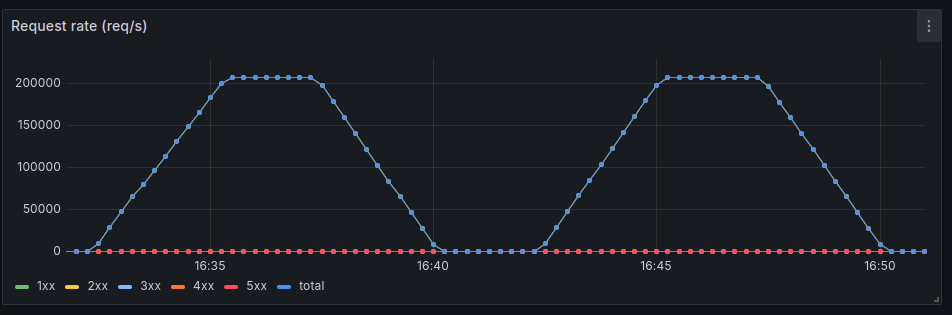
\includegraphics[scale=0.3]{chapter2/chap2-subfigure-example.png}
        \caption{Caption of figure 1}
        \label{fig:chap2-subfigure-example-1}
    \end{subfigure}%
    \begin{subfigure}{0.5\textwidth}
        \centering
        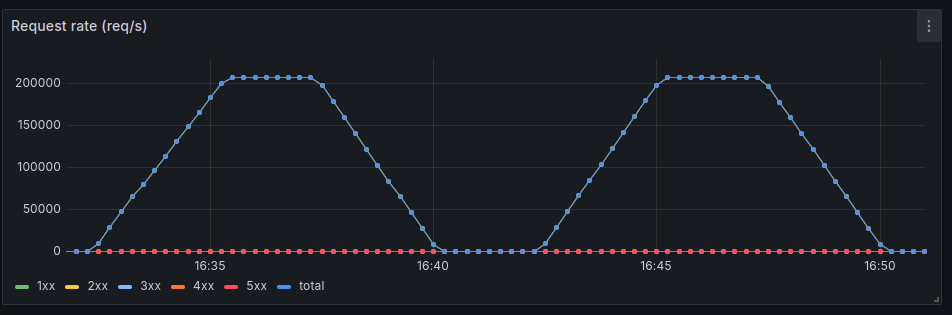
\includegraphics[scale=0.3]{chapter2/chap2-subfigure-example.png}
        \caption{Caption of figure 2}
        \label{fig:chap2-subfigure-example-2}
    \end{subfigure}
    \caption{Mô tả chèn hình ảnh con trong một hình ảnh lớn}
    \label{fig:chap2-subfigure-example}
\end{figure}

\section{Chèn hình ảnh với ghi chú ở bên cạnh}

Chèn hình ảnh toàn trang thì tương đối dễ, ta chỉ việc chèn hình đó với độ thu phóng phù hợp. Phần này trình bày việc chèn các hình ảnh toàn trang và có ghi chú nằm ở vị trí khác so với bình thường.

Hình \ref{fig:img-caption-rotate} minh họa hình ảnh và ghi chú của nó được xoay một góc $90^{\circ}$. Đoạn mã \ref{lst:figure-with-caption-rotate} giúp ta làm được điều này.

\begin{figure}
    \begin{minipage}[c]{0.8\textwidth}
      \centering
      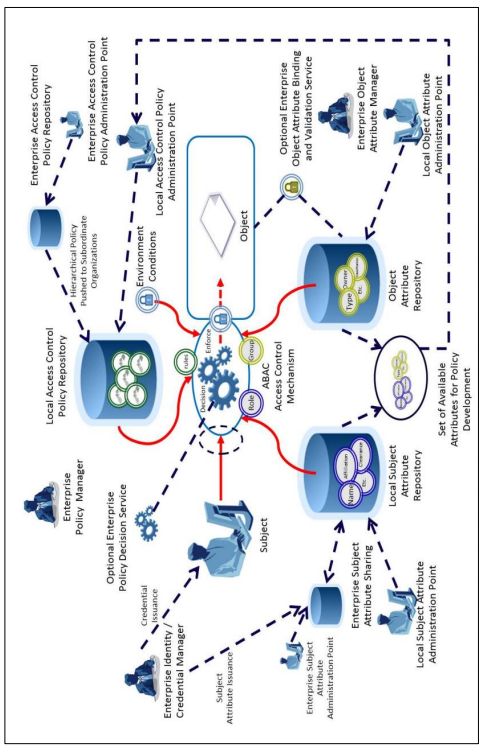
\includegraphics[width=\textwidth]{chapter2/chap2-rotate-figure-example.png} 
    \end{minipage}
    \begin{minipage}[c]{0.1\textwidth}
      \begin{adjustbox}{angle=90,center}
        \begin{minipage}[c]{\textheight}
          \caption{Minh họa chèn hình ảnh với caption xoay $90^{\circ}$}
          \label{fig:img-caption-rotate}
        \end{minipage}
      \end{adjustbox}
    \end{minipage}
\end{figure}

\begin{lstlisting}[language={[LaTeX]TeX}, caption={Chèn hình ảnh với caption xoay $90^{\circ}$}, label={lst:figure-with-caption-rotate}]
\begin{figure}
    \begin{minipage}[c]{0.8\textwidth}
        \centering
        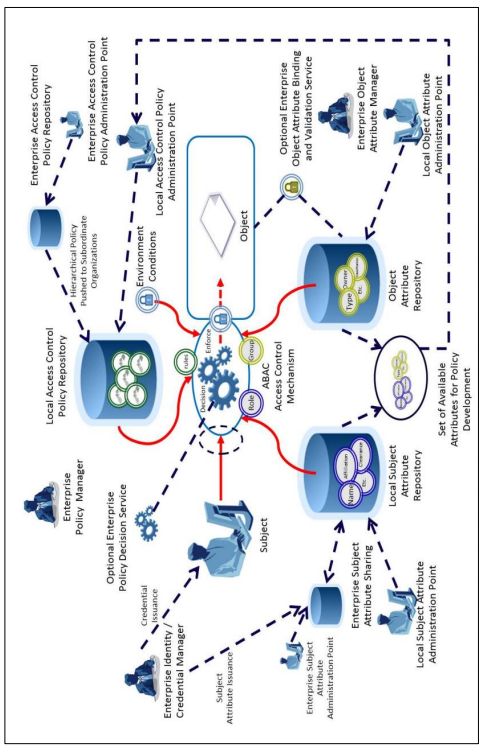
\includegraphics[width=\textwidth]{chapter2/chap2-rotate-figure-example.png} 
    \end{minipage}
    \begin{minipage}[c]{0.1\textwidth}
        \begin{adjustbox}{angle=90,center}
        \begin{minipage}[c]{\textheight}
            \caption{Figure caption}
            \label{fig:img-caption-rotate}
        \end{minipage}
        \end{adjustbox}
    \end{minipage}
\end{figure}
\end{lstlisting}

Trong một số trường hợp, ta chỉ cần caption ở một bên hình ảnh chứ không xoay như hình \ref{fig:img-just-caption-side}, ta chỉ cần thực hiện như đoạn mã \ref{lst:figure-just-caption-side}.

\begin{figure}
    \begin{minipage}[c]{0.7\textwidth}
      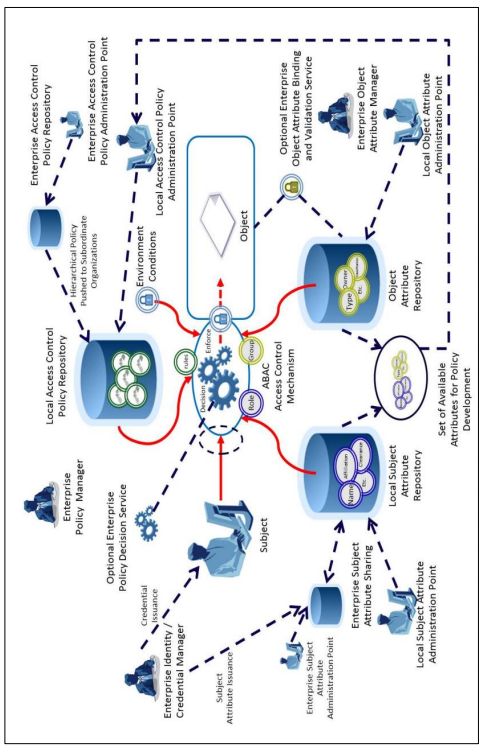
\includegraphics[width=\textwidth]{chapter2/chap2-rotate-figure-example.png}
    \end{minipage}\hfill
    \begin{minipage}[c]{0.2\textwidth}
      \caption{
        Figure caption
      } \label{fig:img-just-caption-side}
    \end{minipage}
\end{figure}

\begin{lstlisting}[language={[LaTeX]TeX}, caption={Chèn hình ảnh với caption ở bên phải $90^{\circ}$}, label={lst:figure-just-caption-side}]
\begin{figure}
    \begin{minipage}[c]{0.7\textwidth}
        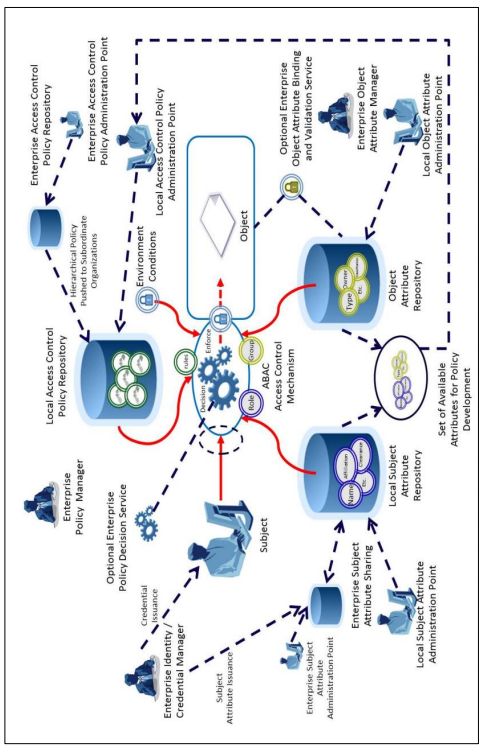
\includegraphics[width=\textwidth]{chapter2/chap2-rotate-figure-example.png}
    \end{minipage}\hfill
    \begin{minipage}[c]{0.2\textwidth}
        \caption{
            Figure caption
        } \label{fig:img-just-caption-side}
    \end{minipage}
\end{figure}
\end{lstlisting}